\documentclass[a4paper,12pt]{article}
\usepackage{graphicx}
\usepackage[left=30mm, right=30mm, top=30mm, bottom=35mm]{geometry}
\usepackage{amsmath}
\usepackage{siunitx}
\usepackage{fancyhdr}
\usepackage{url}
\pagestyle{fancy}
%-------------------------------------------------------------------------------
\lhead{\textbf{Spring 2019}}
\rhead{\textbf{CE394M Advanced Analysis in Geotechnical Engineering}}
\cfoot{\thepage}
%-------------------------------------------------------------------------------

\begin{document}
\begin{centering}
	\textbf{
		Assignment 3: Shape functions\\
		Assigned: 17th February 2020\\
		Due: 28th February 2020\\
	}
\end{centering}

\vspace{1em}
 
\begin{enumerate}

	\item Using the Jupyter notebook for shape function plot the shape functions for linear, quadratic and cubic polynomials with equally spaced nodes. Comment on the suitability of these shape functions for calculating deflection, strain, and curvature.
	
	\item Using the same shape function notebook plot and comment on the suitability of a 5th and a 10th order polynomial shape functions with equally spaced nodes.

	\item Using hand calculations compute and plot the standard shape function for the element shown in Figure 1a.
	
	\item Modify the Jupyter notebook for shape function exercise to compute the shape functions for the elements shown in Figure 1. Compare your result from the  hand calculation with the solution obtained using the Jupyter notebook for Figure 1a. Please try part (1b) with Jupyter notebooks only. Comment on the degree of displacement and strain that can be modeled using these elements:
	\begin{figure}[!h]
		\centering
		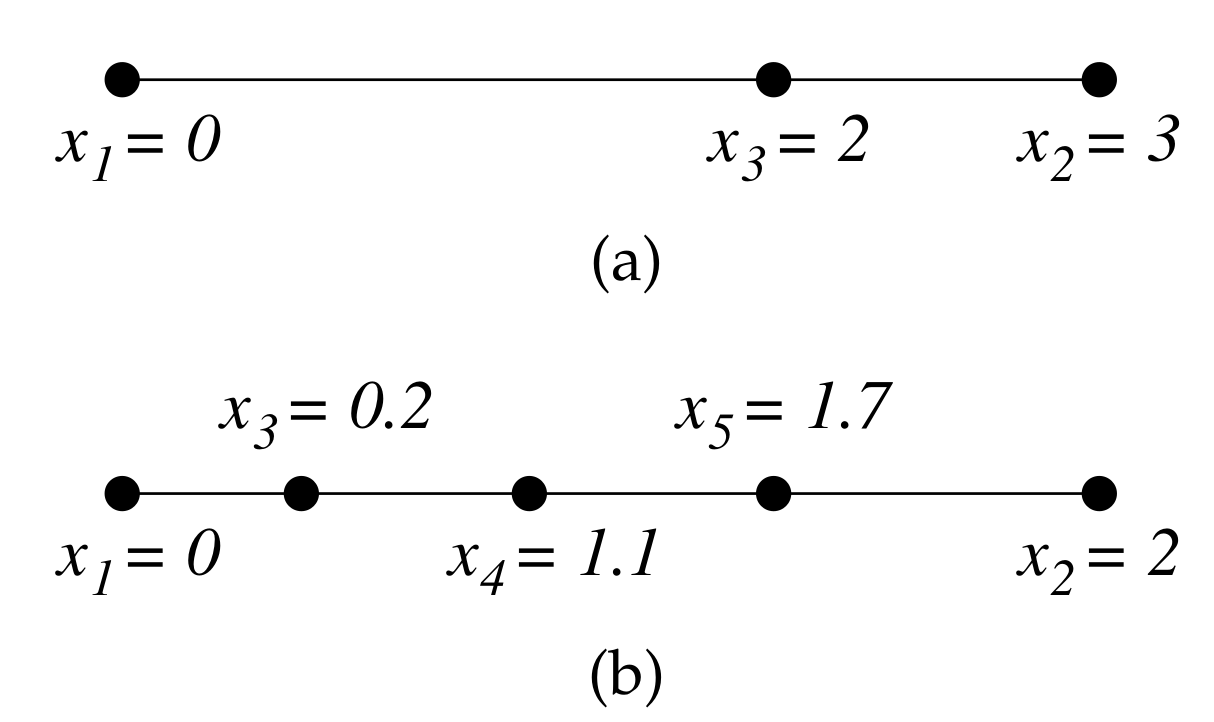
\includegraphics[width=0.5\textwidth]{figs/shapefns.png}
		\caption{1D elements}
	\end{figure}

	\item For a linear element with nodes $x_1 = 0$ and $x_2 = l$, compute the `element mass matrix' $M_e = \int_0^l N^T N dx$. Comment on the mass conservation of the element matrix. The mass matrix derived is called the `consistent mass matrix`. Could you try to derive the equivalent lumped mass matrix? Comment on the suitability of consistent and lumped mass matrices.
	
\end{enumerate}

\end{document}

